% !TeX spellcheck = en_US

\chapter{Implementation}
This chapter describes the technical implementation of the transition process shown in figure \ref{fig:websuite-migration}.

\begin{figure}[H]
	\centering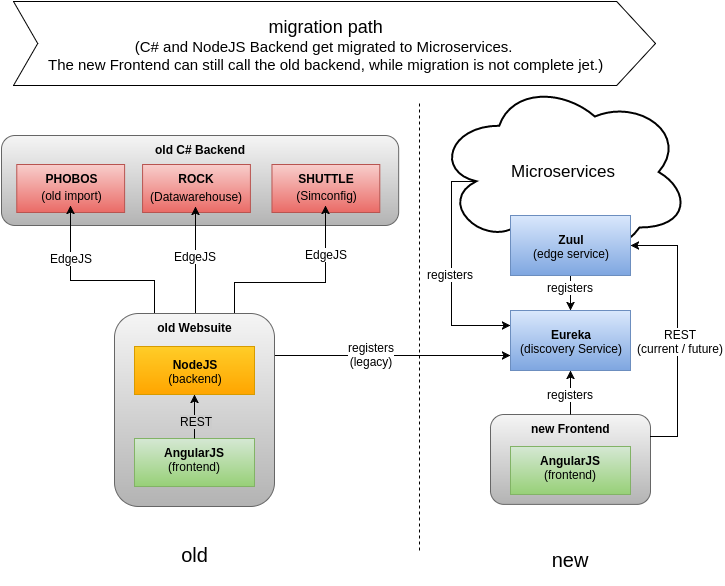
\includegraphics[width=1\textwidth]{res/Websuite_migration}
	\caption{Websuite migration path}
	\label{fig:websuite-migration}
\end{figure}

The old JavaScript stack, containing of an AngularJS frontend and an NodeJS backend with connection to the C$\sharp$ code over EdgeJS was replaced. The NodeJS components were migrated to several micro-services and the frontend was converted to a WebUI micro-service that consists of an AngularJS frontend and a thin layer of NodeJS to host the application.\\
The process of migrating to the new structure is complete and the old monolithic Websuite is not used anymore.



\section{Tooling}
To effectively develop a frontend application, certain talks have to be done, to make the process convenient in development and usable in production. The following topics have to be considered.


\subsection{Dependency management}
Almost every application depends on third-party components. Manually managing dependencies is an error prone tasks and checking them into the version control system clutters the history.\\
This is why the WebUI uses NPM and bower. NPM is responsible for managing NodeJS dependencies that are used for tooling and serving the frontend. Bower takes care of the frontend libraries. Both tools depend on a JSON file that lists the needed dependencies, as well as their required version. This guarantees that any deployment of the app uses the correct versions.

\subsection{Task Runner}
A task runner allows to run various tasks that are used during the development process. The WebUI uses Gulp, which is responsible for executing the following tasks.

\subsubsection{Live reload} Restarts the application and reloads the website inside the browser, once the source code has changed. It is only used for development.

\subsubsection{Browser sync} Synchronizes the active state of all open browser windows. This helps testing cross-browser compatibility in development.

\subsubsection{Combining files} Combines all files of a type (e.g. .js, .html or .css) to one file. This reduces the amount of connections needed to serve the page in production and therefore improves load time.

\subsubsection{Uglifying} Renames variables and functions to single character names to reduce the size of the served files in production.

\subsubsection{minifying} Removes spaces and line-breaks in production, to further reduce the file size in production.


\subsection{Intial Configuration}
The tasks above need to be configured, to match the development work-flow and the used file structure. This initial configuration was created with a tool called \textit{generator-gulp-angular} and modified to match the actual need for the WebUI.



\section{Transition of the Components}
% Describe calls and how things are done.


\subsection{Import}
\begin{figure}[H]
	\centering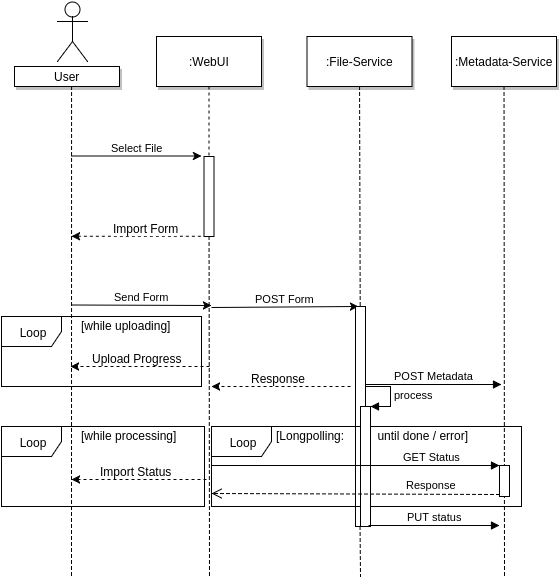
\includegraphics[width=.75\textwidth]{res/Import}
	\caption{Import}
	\label{fig:import}
\end{figure}



\subsection{Data View}



\subsection{Scenario}
\begin{figure}[H]
	\centering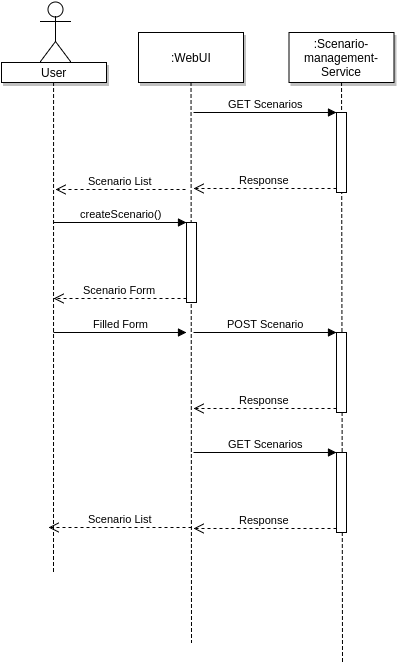
\includegraphics[width=.65\textwidth]{res/Scenario}
	\caption{Scenario}
	\label{fig:scenario}
\end{figure}



\subsection{Mapping}
\begin{figure}[H]
	\centering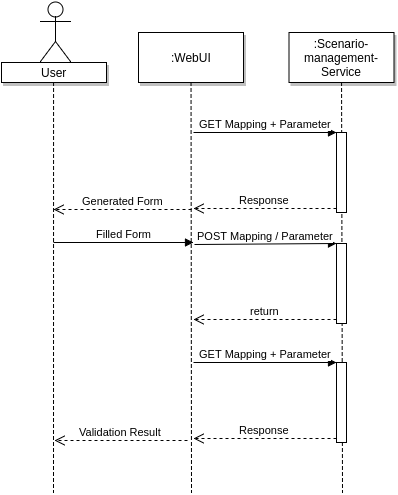
\includegraphics[width=.65\textwidth]{res/Mapping}
	\caption{Mapping}
	\label{fig:mapping}
\end{figure}




\section{Error Handling}
% Display of error messages to the user
% Dashboard to show service availability
